\subsection{GUI}
\label{kap2_6:GUI}
Im Folgenden werden ausschließlich die \ac{GUI}-Elemente dargestellt die für Pflichtfunktionen benötigt werden.\\


\begin{figure}[h]
\centering
\begin{subfigure}{.5\textwidth}
  \centering
  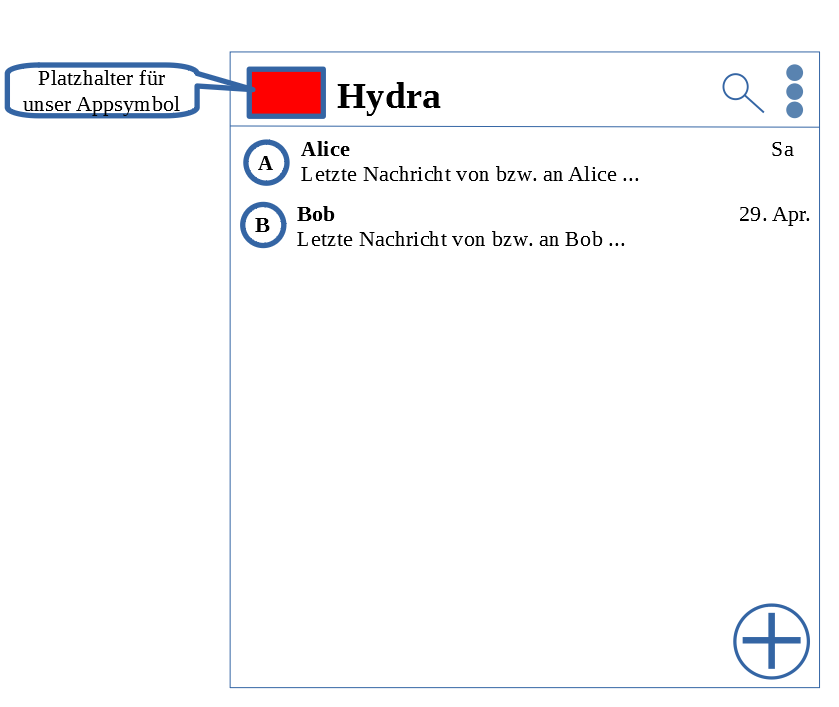
\includegraphics[scale=0.3]{gui/Startseite.png}
  \caption{Startseite}
\end{subfigure}%
\begin{subfigure}{.5\textwidth}
  \centering
  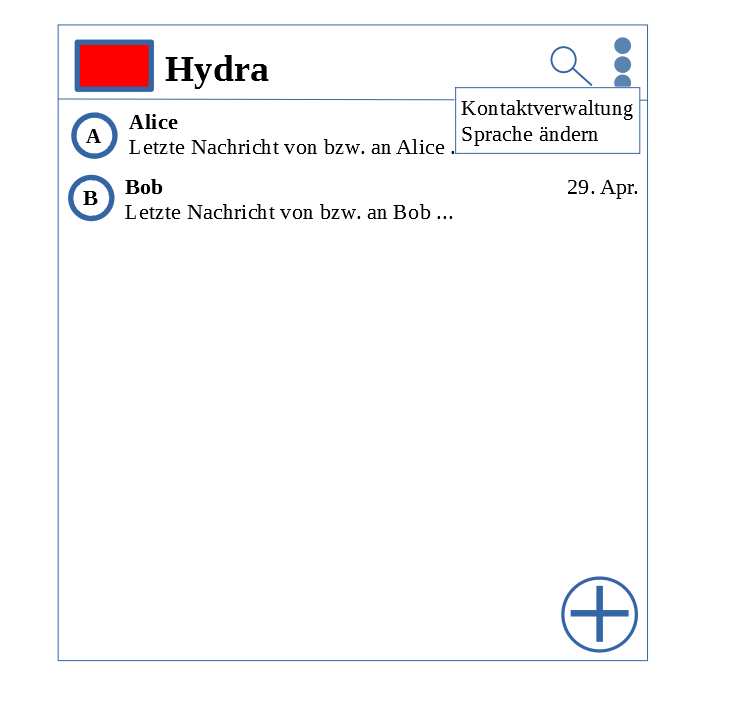
\includegraphics[scale=0.3]{gui/Startseite_mit_Einstellungen.png}
  \caption{Startseite mit Einstellungen}
\end{subfigure}
\caption{GUI Startseite}
\end{figure}

Startseite:\\
Die Lupe oben links ermöglicht die Volltextsuche.\\
Die drei vertikal angeordneten Punkte öffnen die Einstellungen.\\
Anwählen von z.B. Alice öffnet den Chat mit Alice.\\
Das Plus-Symbol unten rechts öffnet die Kontaktverwaltung.\\
\newpage

\begin{figure}[h]
\centering
\begin{subfigure}{.5\textwidth}
  \centering
  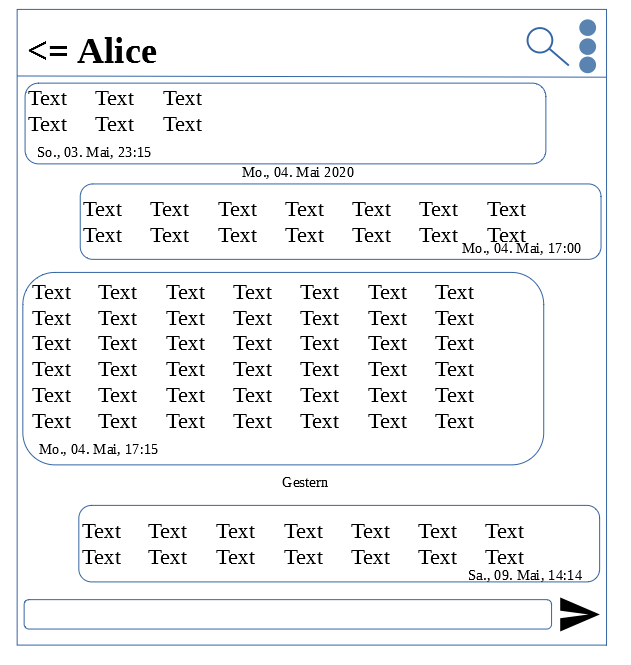
\includegraphics[scale=0.3]{gui/Chatfenster.png}
  \caption{Chatfenster}
\end{subfigure}%
\begin{subfigure}{.5\textwidth}
  \centering
  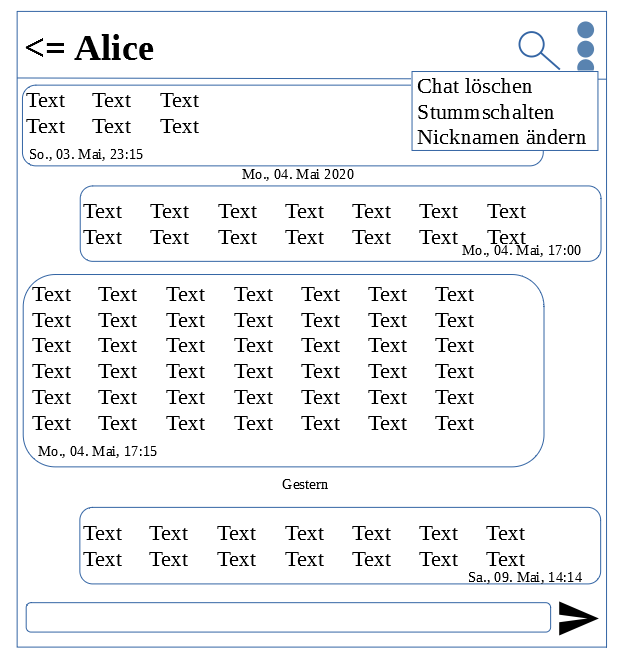
\includegraphics[scale=0.3]{gui/Chatfenster_mit_Einstellungen.png}
  \caption{Chatfenster mit Einstellungen}
\end{subfigure}
\caption{GUI Chatfenster}
\end{figure}

Chatfenster:\\
Die Lupe oben links ermöglicht die Volltextsuche in diesem Chat.\\
Im Chatfenster öffnen die drei vertikal angeordneten Punkte die Chat-Einstellungen.\\
Anwählen der Leiste am unteren Bildschirmrands ermöglicht die Eingabe einer Nachricht.\\
Der Pfeil am unteren rechten Rand versendet die Verfasste Nachricht.\\

\newpage

\begin{figure}[h]
\centering
\begin{subfigure}{.5\textwidth}
  \centering
  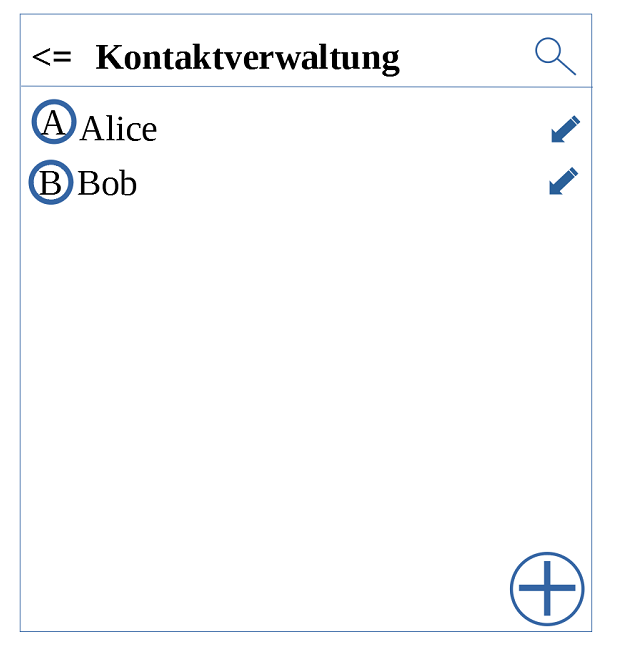
\includegraphics[scale=0.3]{gui/Kontaktverwaltung.png}
  \caption{Kontaktverwaltung}
\end{subfigure}%
\begin{subfigure}{.5\textwidth}
  \centering
  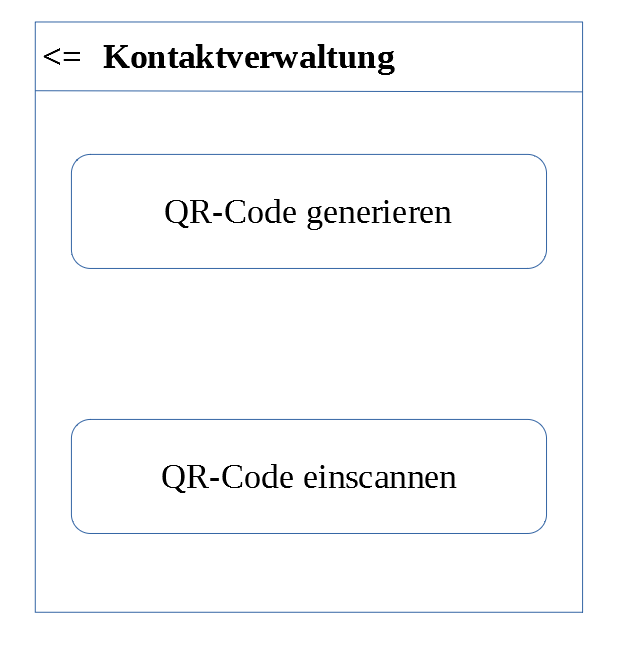
\includegraphics[scale=0.3]{gui/Kontaktverwaltung_QR_Code.png}
  \caption{Kontaktverwaltung QR-Code}
\end{subfigure}
\caption{GUI Kontaktverwaltung}
\end{figure}

Kontaktverwaltung:\\
In der Kontaktverwaltung kann man durch anwählen eines Kontaktes den zugehörigen Chat öffnen bzw. falls noch keiner existiert diesen starten.\\
Der Stift am rechten Rand lässt den Benutzer das Pseudonym des Kontaktes ändern.\\
Das Plus-Symbol unten rechts ermöglicht es dem Benutzer neue Kontakte hinzuzufügen.\\

\begin{figure}[h]
\centering
\begin{subfigure}{.5\textwidth}
  \centering
  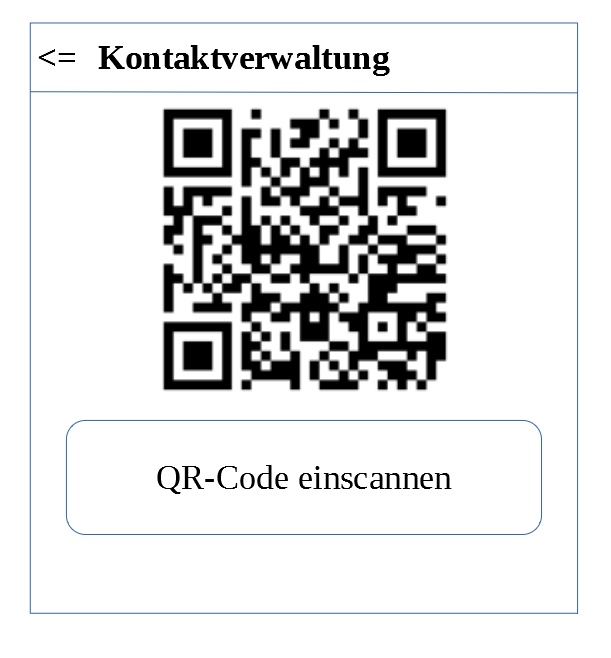
\includegraphics[scale=0.3]{gui/Kontaktverwaltung_QR_Code_generiert.png}
  \caption{Generierter QR-Code}
\end{subfigure}%
\begin{subfigure}{.5\textwidth}
  \centering
  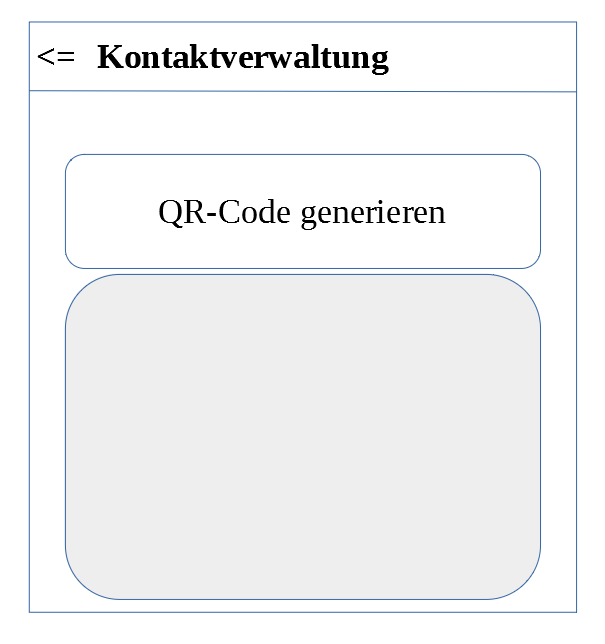
\includegraphics[scale=0.3]{gui/Kontaktverwaltung_QR_Code_einscannen.png}
  \caption{QR-Code einscannen}
\end{subfigure}
\caption{GUI QR-Code}
\end{figure}


